% !TEX root = ../main.tex
\paragraph{Particle Identification}
% --+ PDG PID +-----------------------------------------------------------------
    The Particle Identification (PID) numbering scheme described here was initially introduced by the Particle Data Group (PDG) in 1988 \cite{yost1988}.
    Its purpose is to facilitate communication and data exchange between different generators, simulators, and analysis packages employed in particle physics.
    The system underwent subsequent revisions and adaptations in 1998 to allow for the systematic inclusion of undiscovered and hypothetical particles \cite{particle1998}.
    The PID convention utilised in this thesis is based on the most up-to-date version available at the time of writing, as referenced from the 2020 Review of Particle Physics by the PDG \cite{particle2020}.

% --+ The Event Builder +-------------------------------------------------------
    The Event Builder (EB) is a crucial component within the reconstruction chain, serving multiple functions:
    \begin{itemize}
        \item
            It gathers information from upstream services.
        \item
            It correlates information from sub-detectors to form particles.
        \item
            It implements a general particle identification scheme.
        \item
            It organises the resulting information into a standardised and persistent data bank structure.
    \end{itemize}

    The EB service is executed twice using identical algorithms, first employing hit-based tracks and subsequently using time-based tracks.
    As mentioned previously, the results obtained from the hit-based EB are utilised to initialise time-based tracking.

% --+ Forming particles +-------------------------------------------------------
    In the definition of a reconstructed charged particle within CLAS12, the EB assumes that each reconstructed track in both the FD and the CD will be assigned an identification.
    The corresponding responses from the calorimeter, scintillator, and Cherenkov detectors are then associated with that particle based on geometric coincidences between the detector responses and the track.
    Matching criteria are established, which correspond to the resolution of each specific detector.
    The geometric matching process relies on the Distance of Closest Approach (DOCA) between the track and the detector response.

    A similar procedure is employed for the creation of neutral particles, with the distinction that the seeding is presently performed using unassociated responses from the ECAL for the FD and the CND (or the BAND) for the CD, instead of using tracks.

% --+ Event start time +--------------------------------------------------------
    A start time is assigned to the entire event and serves as the precise reference time for all time-based particle identification procedures.
    The determination of the start time relies on the optimal charged particle candidate in the FD with an associated timing response from the FTOF detector.

    The EB assigns the start time based on the highest energy electron detected in the ECAL.
    If no electron is found in the ECAL, the EB then searches for a positron in the ECAL.
    In the absence of any lepton candidates, the next track in the priority list is a forward-going positive track, which is assumed to be a positive pion ($\pi^+$).
    Finally, if no forward-going positive track is identified, the EB searches for a forward-going negative track, assumed to be a negative pion ($\pi^-$).
    When searching for $\pi^+$ or $\pi^-$ tracks, only the candidate with the highest momentum within each group is considered.

    A parallel event start time is determined from the FT system to facilitate physics analyses and triggers specifically for events where the primary scattered electron is at very forward angles within the FT.

    In such cases, all combinations of charged particles in both the FT and the FD are taken into account.
    The particle in the FT is assumed to be an electron, while all possible hadron mass hypotheses are considered for the FD tracks.
    The combination that exhibits the best time coincidence is selected, and the timing of the resulting FT electron is used to assign the start time.

    A correction to the start time is subsequently applied using the Radio Frequency (RF) signal from the accelerator, in conjunction with the reconstructed event vertex position.
    This correction effectively aligns the event start time with the most accurate measurement of the beam-bunch arrival time at the target.

    The uncorrected measured vertex time of a particle, denoted as $t_v$, can be expressed as follows
    \begin{equation*}
        t_v = t - \frac{P_L}{\beta c},
    \end{equation*}

    Here, $t$ represents the measured time response (e.g., in a scintillator), $P_L$ is the path length between the primary interaction vertex and the corresponding response, and $\beta c$ denotes the speed of the particle.

    Next, we calculate the time difference $\Delta t_{RF}$ between $t_v$ and the nearest beam bunch using the following formula
    \begin{equation*}
        \Delta t_{RF} = t_v + \frac{z_0 - z_v}{c} - t_{RF} - \frac{N}{2f_{RF}},
    \end{equation*}

    In this equation, $z_v$ represents the $z$-coordinate of the event vertex position, $z_0$ is the reference position calibration at the center of the target, and $c$ denotes the speed of light in vacuum.
    $t_{RF}$ and $f_{RF}$ correspond to the measured and calibrated RF time and frequency of the accelerator.
    These values can either be $2.004 \text{ ns}$ and $249.5 \text{ MHz}$, or $4.008 \text{ ns}$ and $499 \text{ MHz}$, respectively.
    During the reconstruction process, these values are obtained from the Run Conditions Database (RCDB).

    Subsequently, the time can be further corrected to the nearest beam bunch using the equation
    \begin{equation*}
        \Delta t^\prime_{RF} = \text{mod}\left(\Delta t_{RF}, \frac{1}{f_{RF}}\right) - \frac{1}{2f_{RF}},
    \end{equation*}

    This correction allows for RF-correction to $t_v$. Thus, we obtain a final RF- and vertex-corrected start time for the event, defined as
    \begin{equation*}
        t' = t_v - \Delta t^\prime_{RF}.
    \end{equation*}

% --+ Charged particle identification +-----------------------------------------
    The subsequent step involves a basic particle identification scheme designed to be flexible enough to accommodate various physics analyses while retaining essential information for future refinement of the criteria.

    \begin{wrapfigure}{r}{0.49\textwidth}
        \centering\frame{
        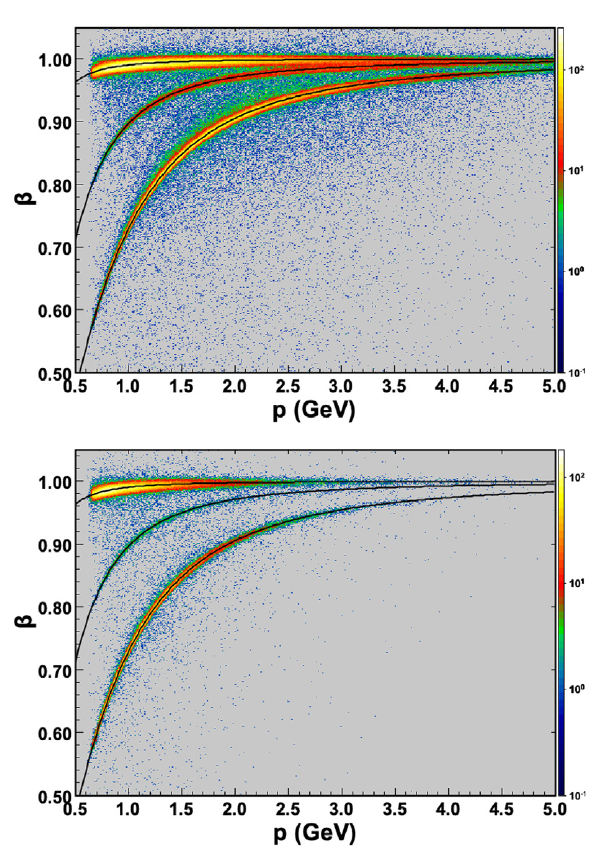
\includegraphics[width=\linewidth]{232pos_pid.png}}
        \caption[Particle $\beta$ vs. momentum for positively charged tracks.]{Particle $\beta$ vs. momentum from simulation data for positively charged tracks with their start time from an electron in the FD (top plot) or in the FT (bottom plot).
        Source: \cite{ziegler2020}.}
        \label{fig::11.232::positive_pid}
    \end{wrapfigure}

    For charged particles, the identification process begins by utilising calorimetry and Cherenkov information to positively identify $e^-/e^+$ candidates in the FD.
    If the measured energy deposition aligns with the expected sampling fraction of the ECAL and the photoelectron response from the HTCC aligns with $\beta \sim 1$, the particle is assigned as an $e^-$ or $e^+$ based on the sign of curvature determined from forward tracking with the DC in the presence of the torus magnetic field.

    The remaining charged particles are then assumed to be hadrons and are assigned an identity solely based on timing information.
    The $p, K, \pi$ candidate with the smallest time residual is selected.
    This time residual is calculated as the difference between the measured flight time of the particle and the flight time computed for a specific mass hypothesis.

    Figure \ref{fig::11.232::positive_pid} presents the $\beta$ vs. momentum distributions for forward-going positively charged hadrons reconstructed using data from the FTOF and DC subsystems.
    The electron is reconstructed either in the FD (top) or in the FT (bottom).
    The computed curves for different mass hypotheses are superimposed on the distributions.

    \begin{wrapfigure}{r}{0.50\textwidth}
        \centering\frame{
        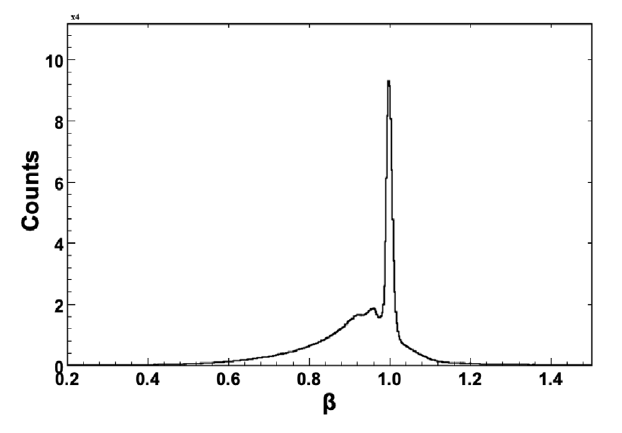
\includegraphics[width=\linewidth]{232n_gamma.png}}
        \caption[$\beta$ distribution of neutrals.]{$\beta$ distribution for neutral particles as measured by the ECAL from simulation data, showing a sharp peak at $\beta = 1$ from photons and a broader, slower distribution from neutrons.
        Source: \cite{ziegler2020}.
        }
        \label{fig::11.232::neutrons_and_gamma}
    \end{wrapfigure}

% --+ Neutral particle identification +-----------------------------------------
    To identify neutral particles, the analysis assumes the presence of only neutrons and photons, distinguished solely by timing and topological information.
    In the FD, the identification is based on the ECAL, while in the CD, it relies on the CND.
    The reconstructed cluster positions of these detectors are used to calculate the particle's travel path from the event vertex, assuming a straight-line trajectory.

    If the measured $\beta$ value is close to $1$, the particle is identified as a photon; otherwise, it is identified as a neutron.
    For photons in the FD, the momentum is determined from the deposited energy and the ECAL sampling fraction \cite{asryan2020}.
    For neutrons, the momentum is assigned based on the measured $\beta$, assuming the mass of a neutron.

    Figure \ref{fig::11.232::neutrons_and_gamma} illustrates an example of the reconstructed $\beta$ values for neutral particles in the FD, demonstrating the separation between photons and neutrons.

% --+ Particle identification performance +-------------------------------------
    A particle identification quality factor, represented as a signed-$\chi^2$ or pull, is assigned based on the contributions from individual detector subsystem responses and their resolutions.
    For $e^-/e^+$ identification, the resolution-normalised distance from the expected ECAL sampling fraction is utilised, while for charged hadrons, the resolution-normalised time difference is employed.
    The resulting information is organised into standardised output bank structures for physics analysis.
    This includes the particle four-vectors, associated detector responses, and global event information such as beam RF and helicity details.

    The accuracy of the currently implemented particle identification algorithm can be estimated by comparing the assigned particle identification with the true identification in Monte Carlo simulations.
    Table \ref{tab::11.232::reconstruction_pid} presents the particle identification matrix for the FD (left) and CD (right).
    The values are derived from simulations involving electron-hadron or electron-photon pairs with hadron and photon momenta ranging from $1$ to $2.5 \text{ GeV}$ and electron momenta ranging from $1$ to $9 \text{ GeV}$.
    The diagonal elements represent cases where the particle is correctly identified, while the off-diagonal elements represent cases of misidentification \cite{ziegler2020}.

    \begin{table}
        \caption{Particle identification matrix for the FD (left matrix) and CD (right matrix).
        The FD matrix is based on simulated hadrons and photons with momentum between $1$ and $2.5 \text{ GeV}$, and electrons up to $9 \text{ GeV}$.
        The CD matrix is based on simulated hadrons with momentum between $0.3$ and $1.1 \text{ GeV}$.
        The diagonal elements are correctly identified, while the off-diagonal elements are misidentified.
        Detector inefficiencies are included.}

        \begin{tabularx}{\textwidth}{XXXXXXX|XXXXX}
            \hline
                     & \multicolumn{6}{l}{\textit{FD Truth}} & \multicolumn{5}{l}{\textit{CD Truth}}  \\
            \cline{2-12}
                     & $e$      & $\pi$ & $K$  & $p$  & $n$  & $\gamma$ &       & $\pi$    & $K$  & $p$  & $n$  \\
            \hline
            $e$      & 0.98     &       &      &      &      &          &       &          &      &      &      \\
            $\pi$    &          & 0.93  & 0.10 & 0.00 &      &          & $\pi$ & 0.84     & 0.14 & 0.00 &      \\
            $K$      &          & 0.03  & 0.80 & 0.00 &      &          & $K$   & 0.11     & 0.80 & 0.01 &      \\
            $p$      &          & 0.03  & 0.02 & 0.98 &      &          & $p$   & 0.03     & 0.04 & 0.95 &      \\
            $n$      &          &       &      &      & 0.66 & 0.01     & $n$   &          &      &      & 0.11 \\
            $\gamma$ &          &       &      &      & 0.14 & 0.95     &       &          &      &      &      \\
            \hline
        \end{tabularx}
        \label{tab::11.232::reconstruction_pid}
    \end{table}
